\documentclass[runningheads,a4paper]{llncs}

\usepackage{amssymb}
\usepackage{amsmath}
\usepackage{todonotes}
\setcounter{tocdepth}{3}
\usepackage{graphicx}

\graphicspath{{pics/}}
\DeclareMathOperator*{\argmax}{arg\,max} 
\DeclareMathOperator*{\argmin}{arg\,min} 

\usepackage{url}
\urldef{\mailsa}\path|alserg@rain.ifmo.ru|
\newcommand{\keywords}[1]{\par\addvspace\baselineskip
\noindent\keywordname\enspace\ignorespaces#1}

\begin{document}

\mainmatter  % start of an individual contribution

% first the title is needed
\title{An algorithm for fast preranked gene set enrichment analysis using 
    cumulative statistic calculation}

% a short form should be given in case it is too long for the running head
\titlerunning{Fast preranked gene set enrichment analysis}

%
\author{Alexey A. Sergushichev}
%
\authorrunning{A.~A.~Sergushichev}
% (feature abused for this document to repeat the title also on left hand pages)

% the affiliations are given next; don't give your e-mail address
% unless you accept that it will be published
\institute{
    Computer Technologies Department, ITMO University, 
    Saint Petersburg, 197101, Russia \\
\mailsa\\
}

%
% NB: a more complex sample for affiliations and the mapping to the
% corresponding authors can be found in the file "llncs.dem"
% (search for the string "\mainmatter" where a contribution starts).
% "llncs.dem" accompanies the document class "llncs.cls".
%

\toctitle{Lecture Notes in Computer Science}
\tocauthor{Authors' Instructions}
\maketitle

\begin{abstract}
Gene set enrichment analysis is a widely used tool for analyzing gene 
expression data. However, current implementations are slow due to a large
number of required samples for the analysis to have a good statistical power.
In this paper we present a novel algorithm, that efficiently reuses
one sample multiple times and thus speeds up the analysis.
We show that it is possible to make hundreds of thousands permutations 
in a few minutes, which leads to very accurate p-values. This, in turn,
allows applying standard FDR correction procedures, which are
more accurate than the ones currently used.
The method is implemented in a form of an R package and 
is freely available at \url{https://github.com/ctlab/fgsea}.

\keywords{gene set enrichment, GSEA, sampling, R package}
\end{abstract}


\section{Introduction}

Gene set enrichment analysis is a very widely used method for analyzing 
gene expression data. It allows to select from an \emph{a priori} defined
list of gene sets those
which have non-random behavior in a considered experiment. Compared
to a similar method of calculating Fisher p-values of overlap statistic
it does not require an arbitrary thresholding. This also allows the method
to identify pathways that contain many co-regulated genes but with small 
individual effects.

The method has a major drawback of being relatively slow. Because analytical
from of the null distribution for the used gene set enrichment statistic 
is not known, empirical null distribution has to be calculated. That can be
done in a straightforward manner by sampling random gene sets. However,
a big number of gene sets are usually tested simultaneously. This leads to
a requirement of a large number of samples 
for the test to have a good statistical power after a correction for 
multiple testing.

In the original paper \cite{Subramanian2005} Subramanian et al. developed
an ad-hoc method for multiple testing correction.
However, the developed method is approximate for the commonly used
parameters and it is unclear how accurate it is.

Here we present a fast gene set enrichment analysis (FGSEA) method 
which is much faster than the original method \cite{Subramanian2005}
in finding nominal p-values. The method is based on an
algorithm to calculate cumulative gene set enrichment statistic
values, which allows to rapidly calculate multiple sample
statistic values from a single sample. Ability to get accurate nominal p-values
achieved by the method in a reasonable time leads to using
well-developed general methods for multiple testing
correction such as Bonferroni or Benjamini-Hochberg.

The rest of the paper is structured as follows. First,
in section~\ref{section_definitions} we formally define
gene set enrichment statistic and introduce related definitions.
In section~\ref{section_mean}
we explain the idea of the algorithm on a simple mean statistic.
Then, in section~\ref{section_gsea} we show how GSEA statistic
can be interpreted geometrically and present the algorithm
for fast computation of cumulative values that 
follows from such interpretation. Finally,
in section~\ref{section_experiments} we show how the algorithm works
in practice and how it is compared to the reference implementation.

\section{Definitions}\label{section_definitions}

The preranked gene set enrichment analysis takes as input two objects:
an array of gene statistic values $S$ and a list of query gene sets $P$.
The goal of the analysis is to determine which of the gene sets from $P$
has a non-random behavior.

The gene statistic array $S$ of the size $|S| = N$ for each gene
$i$,  $1 \le i \le N$, contains a value $S_i \in \mathbb{R}$ 
that characterises the gene behavior in a considered process.
Commonly, if $S_i > 0$ the expression of gene $i$ goes up in a treatment
compared to 
control and $S_i < 0$ means that the expression goes down. Absolute value 
$|S_i|$ represents a magnitude of the change. Array $S$ is
sorted in a decreasing order: $S_i > S_j$ for $i < j$. 
The value of $N$ in practice is about 10000--20000.

The list of gene sets $P$ of length $|P| = m$ usually contains groups of 
genes that are commonly regulated in some biological process.
In this
paper we assume that all gene sets $p \in P$ have a size upper bound
of $K \approx 500$ genes: $|p| \le K$, $\forall p \in P$.

To quantify a co-regulation of genes in a gene set $p$ Subramanian et al.
introduced a gene set enrichment score function $s_r(p)$ that uses
gene rankings (values of $S$).
The more positive is the value of 
$s_r(p)$ the more enriched the gene set is in positively-regulated
genes $g$ with $S_g > 0$, accordingly, negative $s_r(p)$ corresponds
to enrichment of negatively regulated genes.

Value of $s_r(p)$ can be calculated as follows. Let $k = |p|$, 
$\mathrm{NS} = \Sigma_{i \in p} |S_i|$. Let also $\mathrm{ES}$ be an array 
specified by the following formula: 
\[ \mathrm{ES}_i = \begin{cases} 
        0 & \text{ if } i = 0, \\
        \mathrm{ES}_{i-1} + \frac{1}{\mathrm{NS}} |S_i| & \text{ if } 1 \le i \le N  \text{ and } i \in p, \\
        \mathrm{ES}_{i-1} - \frac{1}{N-k} & \text{ if } 1 \le i \le N \text{ and } i \not \in p.
   \end{cases}
\]
The value of $s_r(p)$ corresponds to the largest by absolute value entry
of $\mathrm{ES}$:
\[
s_r(p) = \mathrm{ES}_{i^*} \text{, where } i^* =  \argmax_i |\mathrm{ES}_i|.
\]

For each $p \in P$ we need to find the enrichment statistic value
and to calculate a p-value of this not to be random. 
To calculate a p-value for gene set $p$ we can obtain an empirical 
null distribution
by sampling $n$ random gene sets of the same size as $p$. 

Such straightforward implementation takes $\Theta(mnK \log K)$ time.
For each of $m$ gene sets we need to perform $n$ permutations for all
of which we need to calculate enrichment statistic value, that
can be done in $\Theta(K \log K)$ time.

\section{Cumulative statistic calculation for mean statistic}\label{section_mean}

Let first describe the idea of the proposed algorithm on a simple statistic
of mean rank $s_m$:
\[
    s_m(p) = \frac{1}{|p|} \Sigma_{i \in p} S_i.
\]

The idea of the algorithm is to reuse sampling for different query gene sets.
This can be done due to the fact that for an estimation of null distributions
samples have to be independent only for a specific gene set size.
Samples can be dependent between different sizes.

Instead of generating $nm$ independent random gene set for each
permutation and each gene set we will generate only $n$ radom
gene sets of size $K$. Let $\pi_i$ be an $i$-th random gene set of 
size $K$. From that gene set we can generate gene sets
for a all the query pathways $P_j$ by using its prefix: $\pi_{i,j}=
\pi_i[1..|P_j|]$.

The next step is to calculate enrichment scores for all generated
gene sets $\pi_{i,j}$. Instead of 
calculating enrichment scores separately for each gene set
we will calculate simultaneously scores for all $\pi_{i,j}$ for a fixed
$i$. Using a simple procedure it can be done in $\Theta(K)$ time.

Let us find enrichment scores for all prefixes of $\pi_i$. This
can be done by element-wise dividing of cumulative sums array
by the length of the corresponding prefix:
\[
    s_m(\pi_i[1..k]) = \frac{1}{k} \Sigma_{i \in \pi_i[1..k]} S_i.
\]

Selecting only the required prefixes takes an additional $\Theta(m)$ time. 

The described procedure allows to find p-values
for all query gene sets in $\Theta(n(K+m))$ time.
This is about $\min(K, m)$ times faster than the straightforward procedure.

\section{Cumulative statistic calculation for GSEA statistic}\label{section_gsea}

For the GSEA statistic we use the similar idea: we will also be sampling only 
gene sets of size $K$ and from that sample will calculate
statistic values for all the other sizes. However, calculation of the 
cumulative statistic values for the subsamples is more complex
in this case.

In this section we only be considering positive mode of 
enrichment statistic 
$s^+_{r}$. It can be defined as follows:
\[
s^+_r(p) = \mathrm{ES}_{i^+} \text{, where } i^+ =  \argmax_i \mathrm{ES}_i.
\]
Calculation of $s^-_{r}(p) = \mathrm{ES}_{i^-}$ 
for $i^- =  \argmin_i\mathrm{ES}_i$
is very similar. From these two values it easy to find 
value of $s_r(p)$, which is equal to $s^+_r(p)$ if
$|s^+_r(p)| > |s^-_r(p)|$ or $s^-_r(p)$ otherwise.


\subsection{Geometric interpretation of GSEA statistic}

It is helpful to look at GSEA statistic from a geometric point of view.
Let us consider $N+1$ points (Fig.~\ref{fig_gsea_stat}) with coordinates $(x_i, y_i)$ for $0 \le i \le N$
such that:
\begin{align}
    \label{eq_simple_0}
    (x_0, y_0) &= (0, 0), & \\ 
    \label{eq_simple_x}
    x_i &= x_{i-1} + [i \not \in p],       &\forall i \in 1..N, \\
    \label{eq_simple_y}
    y_i &= y_{i-1} + [i \in P] \cdot |S_i| &\forall i \in 1..N.
\end{align}

\begin{figure}[h]
    \centering
    { 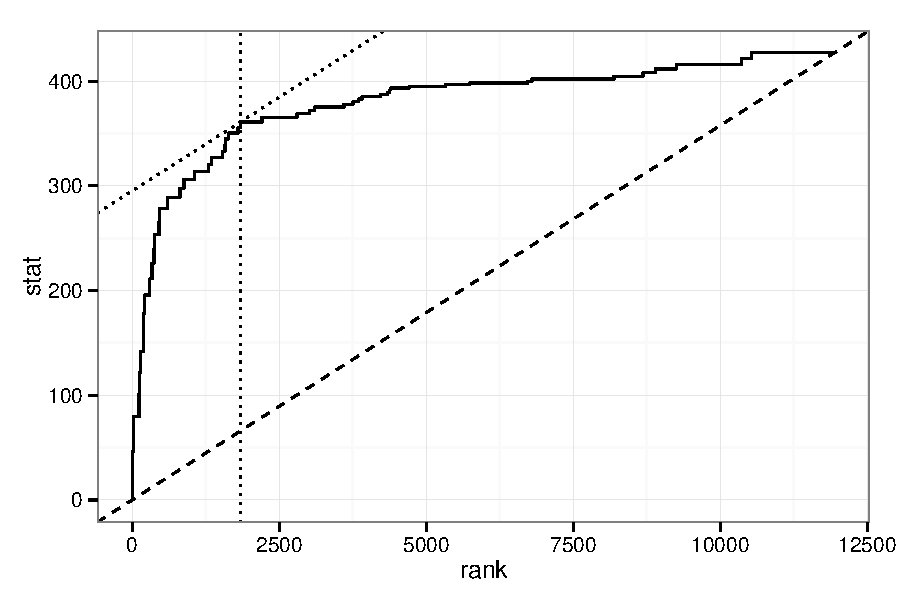
\includegraphics[width=0.75\textwidth]{gsea_stat.pdf} }
    \caption{A graph that corresponds to a calculation of GSEA 
    statistic. Each breakpoint on a graph corresponds to 
    a gene present in the pathway. 
    Dotted line cross at a point which is the farthest
up from a diagonal (dashed line). This point correspond to gene $i^+$, 
where the maximal value of $\mathrm{ES}_i$ is reached}%
    \label{fig_gsea_stat}%
\end{figure}

The calculation of $s^+_r$ corresponds to finding the point
farthest up from a diagonal $\left((x_0, y_0), (x_N, y_N)\right)$. 
Indeed, it is easy to see that $x_N = N - |p| = N - k$ and
$y_N = \Sigma_{j \in p} |S_j| = \mathrm{NS}$,
while the individual enrichment scores $\mathrm{ES}_i$ 
can be calculated as 
$\mathrm{ES_i} = \frac{1}{NS} y_i - \frac{1}{N - k} x_i$.
Value of $\mathrm{ES_i}$ is proportional to the directed distance from 
the line going through $(x_0, y_0)$ and $(x_N, y_N)$ 
to the point $(x_i, y_i)$.

Let us fix a sample $\pi$ of length $K$.
To efficiently calculate cumulative values $s^+_r(\pi[1..k])$ for $k \le K$ we
need a fast method of updating the farthest point
when a new gene is added. In that case we can add genes
from $\pi$ one by one and calculate values $s^+_r(\pi[1..k])$ 
from the corresponding maximal distances.

Because we are calculating values for $\pi[1..k]$ for $k \le K$
we know in advance which $K$ genes will be added.
This allows us to consider $K+1$ points instead of $N+1$ for each iteration 
$k$. Let array $o$ contains order of genes in $\pi$, that is $\pi_{o_1}$
is minimal among $\pi$, $\pi_{o_2}$ is second minimal and so on.
The coordinates can be calclated as follows:
\begin{align}
    \label{eq_collapsed_0}
    (x^k_0, y^k_0) &= (0, 0), & \\ 
    \label{eq_collapsed_x}
    x^k_i &= x^k_{i-1} + \pi_{o_i} - \pi_{o_{i-1}} - \left[o_i \le k\right],       &\forall i \in 1..K, \\
    \label{eq_collapsed_y}
    y^k_i &= y^k_{i-1} + \left[o_i \le k \right] \cdot |S_i|, &\forall i \in 1..K,
\end{align}
where we set $\pi_{o_0}$ to be zero.

It can be shown that finding the farthest up point among 
\eqref{eq_collapsed_0}--\eqref{eq_collapsed_y} is
equivalent to finding the farthest up point among 
\eqref{eq_simple_0}--\eqref{eq_simple_y} 
with $(x^k_i, y^k_i)$ being equal to $(x_{\pi_{o_i}}, y_{\pi_{o_i}})$
calculated for $p = \pi[1..k]$.

Consider $x_{\pi_{o_i}} - x_{\pi_{o_{i-1}}}$. By the definition of $x$ 
it is equal to:
\begin{multline*}
    x_{\pi_{o_i}} - x_{\pi_{o_{i-1}}} = 
        \sum_{i=1}^{\pi_{o_i}} [i \not \in \pi [1..k]] - 
        \sum_{i=1}^{\pi_{o_{i-1}}} [i \not \in \pi [1..k]] =  
        \sum_{i=\pi_{o_{i-1}} + 1}^{\pi_{o_i}} [i \not \in \pi [1..k]] = \\
        \pi_{o_i} - \pi_{o_{i-1}} - \sum_{i=\pi_{o_{i-1}} + 1}^{\pi_{o_i}} [i \in \pi [1..k]].
\end{multline*}

By the definition of $o$, in the interval 
$[\pi_{o_{i-1}} + 1, \pi_{o_{i}} -1]$ there are no genes from $\pi$ and,
thus, from $\pi[1..k]$. Thus we can replace sum with its last member:
\[
    x_{\pi_{o_i}} - x_{\pi_{o_{i-1}}} = 
        \pi_{o_i} - \pi_{o_{i-1}} - [\pi_{o_i} \in \pi [1..k]] = 
        \pi_{o_i} - \pi_{o_{i-1}} - [o_i \le k].
\]

We got the same difference as in \eqref{eq_collapsed_x}.

Now consider $y_{\pi_{o_i}} - y_{\pi_{o_{i-1}}}$. By the definition of $y$ 
it is equal to:
\[
    y_{\pi_{o_i}} - y_{\pi_{o_{i-1}}} = 
        \sum_{i=1}^{\pi_{o_i}} [i \in \pi [1..k]] \cdot |S_i| - 
        \sum_{i=1}^{\pi_{o_{i-1}}} [i \in \pi [1..k]] \cdot |S_i| =  
        \sum_{i=\pi_{o_{i-1}} + 1}^{\pi_{o_i}} [i \in \pi [1..k]] \cdot |S_i|.
\]

Again, in the interval $[\pi_{o_{i-1}} + 1..\pi_{o_{i}} -1]$ 
there are no genes from $\pi[1..k]$. Thus we can replace the sum with only the
last member:
\[
    y_{\pi_{o_i}} - y_{\pi_{o_{i-1}}} = 
        [\pi_{o_i} \in \pi [1..k]] \cdot |S_i| = 
        [o_i \le k] \cdot |S_i|.
\]

We got the same difference as in \eqref{eq_collapsed_y}.

We do not need to consider other points, because points 
$o_{i-1}..o_i-1$ have the same $y$ coordinate
and $o_{i-1}$ is the leftmost of them. Thus, when at 
least one gene is added the diagonal 
$\left((x_0, y_0), (x_N, y_N)\right)$ is not horizontal and
$o_{i-1}$ is the farthest point among $o_{i-1}..o_i-1$.


\subsection{Square root decomposition}


Let consider what happens when gene $\pi_k$ is added to query set $\pi[1..k-1]$ 
(Fig.~\ref{fig_gsea_update}).
Let $r_k$ be a rank of gene $\pi_k$ among genes $\pi$,
then 
coordinate of points $(x_i, y_i)$ for $i < r_k$ 
do not change, while all $(x_i, y_i)$ for $i \ge r_k$ are changed on
$(\Delta_x,\Delta_y) = (-1, |S_{\pi_k}|)$.

\begin{figure}[h]
\begin{center}
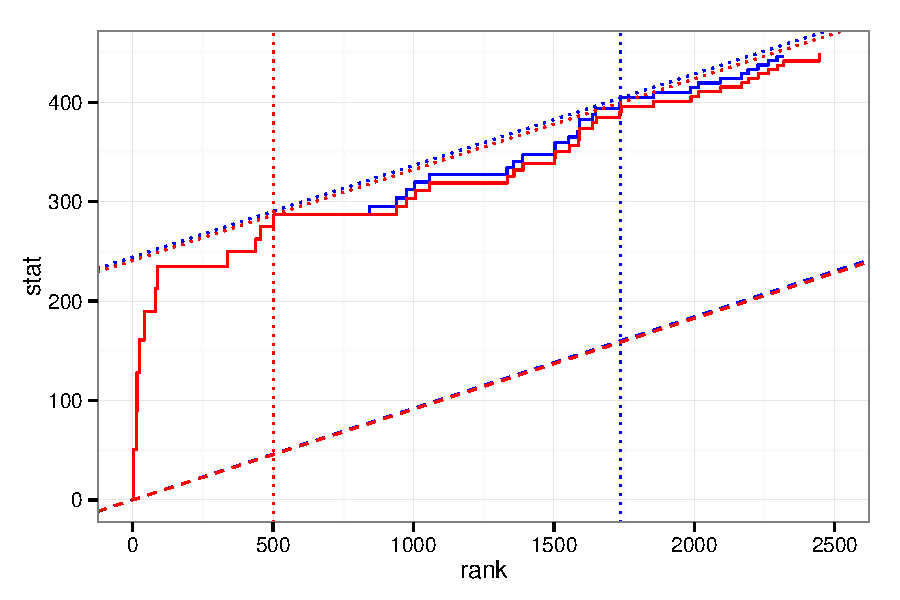
\includegraphics[width=0.7\textwidth]{gsea_update.pdf}
\end{center}
\caption{
    Update of a GSEA graph when gene $\pi_k \approx 800$ is 
    added. Only a fragment is shown. Black graph corresponds
    to the GSEA graph for gene set $\pi[1..k-1]$, 
    gray graph corresponds to $\pi[1..k]$.
    A part of the graph to left of $x=x_{r_k}$ does not change and 
    the other part is shifted to the top-left corner. The diagonal
    $\left((x_0, y_0), (x_N, y_N)\right)$ is rotated
    counterclockwise.
  }\label{fig_gsea_update}
\end{figure}

To make fast incremental updates we will decompose the problem into
multiple smaller ones. For simplicity we assume that $K+1$ is an exact
square of an integer $b$. Let split $K+1$ points into $b$ consecutive 
blocks of the size $b$: 
$\{(x^k_0, y^k_0), ..., (x^k_{b-1}, y^k_{b-1})\}$,
$\{(x^k_b, y^k_b), ..., (x^k_{2b-1}, y^k_{2b-1})\}$ and so on.

For each of $b$ blocks we will store and update the farthest up point
from the diagonal. When we know for each block its farthest point
we can find the globally farthest point by a simple pass in $O(b)$ time.

Next, we show how to update the farthest points in blocks in amortized time
$O(b)$. This taken together with one $O(b)$ pass will get us an algorithm
to update the globally farthest point in amortized $O(b)$ time.

Below we use $c = \lfloor r_k / b \rfloor$ as an index of a block where gene
$\pi_k$ belongs.

First, we describe the procedure to update points coordinates. 
We will store $x_i$ coordinates using two vectors: $B$ of size $b$
and $D$ of size $K + 1$, such that $x_i = B_{i / b} + D_i$.
When gene $\pi_k$ is added all $x_i$ for $i \ge r_k$ are decremented by one.
To reflect this we will decrement all $B_j$ for $j > c$ and decrement
all $D_i$ for $r_k \le i < cb$. It is easy to see that it takes $O(b)$ 
time. After this update procedure we can get value $x_i$ in $O(1)$ time.
The same procedure is applied for $y$ coordinates.

Second, for each block we will maintain an upper part of its convex hull.
Having convex hull is useful because the farthest point in block always
lays on its convex hull.
All blocks except $c$ have the points either not changed or
shifted simultaneously on the same value. That means that lists of points
on the convex hulls for these blocks remain unchanged. For the block $c$
we can reconstruct convex hull from scratch using Graham scan algorithm.
Because the points are already sorted by $x$ coordinate, this
reconstruction takes $O(b)$ time. In total, it takes $O(b)$ time
to update the convex hulls.

Third, the farthest points in blocks can be updated using the stored convex
hulls. Consider a block where the convex hull was not changed (every block
except, possibly, block $c$). Because diagonal always rotates in the same
counterclockwise direction, the farthest point in block on iteration $k$
either stays the same or moves on the convex hull to the left of 
the farthest point on the $(k-1)$-th iteration.
Thus, for each such block we can compare current farthest
point with its left neighbor on the convex hull and update the point if
necessary. It is repeated until the next neighbor is closer to the 
diagonal than the current farthest point. In the block $c$ we just 
find the farthest point in a single pass by the points on the convex hull.

Using potential method we can show that the updating farthest points
takes $O(b)$ amortized time. Let a potential after adding $k$-th
gene $\Phi_k$ be a sum of relative indexes of the farthest points
for all the blocks. As there are $b$ blocks of size $b$ the sum of relative
indexes lies between 0 and $b^2$. Thus, $\Phi_k = O(b^2)$. For an 
update of all $b-1$ blocks except $c$ we need to make $t_k=b-1+z$ 
operations of comparing two points,
where $z$ is the number of times the farthest points were updated. 
This can take up to $\Theta(b^2)$ time in the worst case.
However, it can be noticed, that 
potential change $\Phi_k-\Phi_{k-1}$ is
equal to $-z + O(b)$: the sum of indexes is decreased by a number of 
times the farthest points were updated plus $O(b)$ for the block
$c$ where the index can go from 0 to $b-1$.
This gives an amortized cost of $k$-th iteration to be $a_k = t_k + \Phi_k - \Phi_{k-1} = 
b - 1 + z -z + O(b) = O(b)$. The total real cost of $K$ iterations 
is $\sum_{k=1}^K a_k + \Phi_0 - \Phi_K = O(Kb) + O(b^2) = O(Kb)$,
which means amortized cost of one iteration to be $O(b)$.

Taken together the algorithm allows to find all cumulative
enrichment scores $s_r(\pi[1..k])$ in $O(Kb) = O(K\sqrt{K})$ time.
The straightforward implementation of calculating cumulative
values from scratch would take $O(KK\log K)$ time. Thus,
we have improved the performance $O(K \frac{\log K}{\sqrt{K}})$ times.

\subsection{Implementation details}

We also implemented an optimization that 
does not build convex hull from scratch for a changed block $c$,
but only updates the changed points. This does not influence on
asymptotic performance, but decreases the constant factor.

First, we start updating convex hull from position $r_k$ and
not from 1. To be able to do this, we have an array $\tt{prev}$ that for
each gene $g \in \pi$ stores a previous point on a convex hull
if $g$ were the last gene in the block. This actually is the same as 
the top of the stack in Graham algorithm and represent
the algorithms state for any given point. 
As all points $h$ to the left of $g$ are not changed $\mathtt{prev}_h$
also remains unchanged and need not to be recalculated.

Second, we stop updating the hull, when we reach the point on the
previous iteration convex hull.
We can do this because every point
to the left of $g$ is rotated counterclockwise of any point to the 
right of $g$, which means that the first point on the convex
hull right of $g$ on $(k-1)$-th iteration remains being a convex hull point
at $k$-th iteration.

\section{Experimental results}\label{section_experiments}

To assess the algorithm performance we ran the algorithm 
on a T-cells differentiation dataset \cite{Wei2009}.
The ranking was obtained from differential gene expression analysis
for Naive vs. Th1 states using \emph{limma} \cite{Ritchie2015}.
From that results we selected 12000 genes with the highest
mean expression levels.

As a pathway databases we used Reactome database \cite{Joshi-Tope2005}.
There were 586 gene sets that had overlaps with the selected genes
of the size 15 to 500 (common gene set size limits for preranked 
gene set enrichment analysis).

We compared the algorithm to the reference GSEA implementation~\cite{Subramanian2005}
version~2.1.

Experiments were run on an Intel Core i3 2.10GHz processor. Both methods
were run in one thread.

We ran reference GSEA with default parameters. The permutation number 
was set to 1000, which means that for each input gene set 1000 independent
samples were generated. The run took 100 seconds and resulted
in 79 gene sets with GSEA-adjusted FDR q-value of less than $10^{-2}$. All
significant gene sets were in a positive mode.

First, to get a similar nominal p-values accuracy we ran FGSEA algorithm on
1172 permutations in total ($2\cdot586$: 2 more permutations for each 
additional pathway). This took 3 seconds, but resulted
in no significant hits due to multiple testing correction. The same
effect required GSEA authors to develop a custom method approximate FDR correction.

Second, to get a similar number of significant hits FGSEA
was run with 5860 total permutations.
It took 6 seconds and resulted in 
76 gene sets with BH-adjusted p-value of less than $10^{-2}$. Is is important
to note, that, unlike for GSEA, 3 of these 76 gene sets were in a negative mode.

Last, we ran FGSEA with a similar total running time. Withing 100 seconds
FGSEA was able to do 117200 permutations. This resulted in
78 gene sets with BH-adjusted p-value of less than $10^{-2}$ (3 sets
were in negative mode). The minimal nominal p-value was $1.05\cdot10^{-5}$. 

\section{Conclusion}

Preranked gene set enrichment analysis is a widely used tool in analysis of
gene expression data. However, current implementations are slow due to 
a lot of sampling. Here we present an algorithm that allows to decrease
the number of required samples while keeping the same accuracy 
of nominal p-values. This allows to achieve more accurate p-values
in a faster time. Consequently, gene sets can be ranked more
precisely in the results and, which is even more important, 
standard multiple testing
correction methods can be applied instead of approximate ones
as in \cite{Subramanian2005}. 

\section*{Availability}\label{secion_availability}

The FGSEA method implemented as a package for R and is available at 
\url{https://github.com/ctlab/fgsea} along with the example data
and corresponding results.

\section*{Acknowledgements}\label{secion_acknowledgements}

This work was supported by Government of Russian Federation Grant 074-U01.

The author thanks Gennady Korotkevich for the idea of the algorithm.

\bibliography{mendeley}{}
\bibliographystyle{splncs03}

\end{document}
